%% -----------------------------------------------------------------------------
Interpreting the numeric summaries and aggregations of the preceding section
demands an intuitive understanding of what blame trails look like in practice.
A concrete example of blame trails and programmer modes is a good basis for
synthesizing this kind of intuition.

\begin{figure}
{
  \definecolor{trans-fb}{RGB}{215, 48, 31}
  \definecolor{trans-lb}{RGB}{252, 141, 89}
  \definecolor{trans-exn}{RGB}{253, 204, 0}
  \definecolor{erasure}{RGB}{119, 87, 254}

  \newcommand\config[1]{\begin{minipage}{0.09\textwidth}\centering\includegraphics[width=\linewidth]{Images/#1}\end{minipage}}
  \newcommand\runtimeError{\begin{minipage}{0.03\textwidth}\centering
\includegraphics[width=\linewidth]{Images/runtime-error}\end{minipage}}
  \newcommand\checkFailure{\begin{minipage}{0.03\textwidth}\centering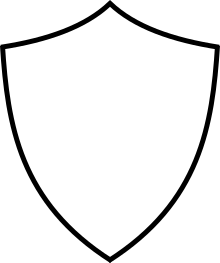
\includegraphics[width=\linewidth]{Images/check-failure-plain}\end{minipage}}
  \newcommand\blameFinger{\begin{minipage}{0.02\textwidth}\centering\vspace{0.25em}\includegraphics[width=\linewidth]{Images/finger}\end{minipage}}
  \newcommand\typeError{\scalebox{1.5}{$\tau_{\hspace{-0.1em}\times}$}}
  \newcommand\success{\textcolor{black!30!green}{\checkmark}}
  \newcommand\fail{\textcolor{red}{\sffamily x}}
  \footnotesize
\centering
\begin{tabular}{l|ccl|ccl|cc|c}
\multicolumn{3}{c}{\begin{minipage}{0.25\textwidth}\centering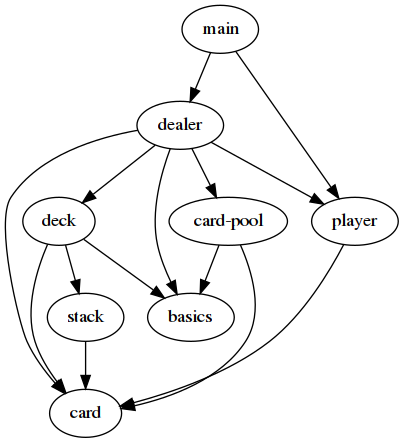
\includegraphics[width=\linewidth]{Images/take5-module-graph}\end{minipage}} &
\multicolumn{7}{c}{\begin{minipage}{0.69\textwidth}\centering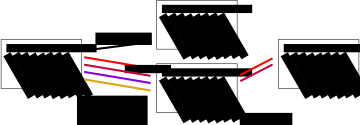
\includegraphics[width=\linewidth]{Images/trails-example}\end{minipage}} \\
\multicolumn{3}{c}{\begin{minipage}{0.25\textwidth}\centering the dependency graph\end{minipage}} &
\multicolumn{7}{c}{\begin{minipage}{0.69\textwidth}\centering the paths taken by each mode through the configuration lattice\end{minipage}} 
\vspace{1em} \\
\end{tabular}

\begin{tabular}{l|ccl|ccl|cc|c}
 & \textbf{Root} &  &  & \textbf{Step 1} &  &  & \textbf{Step 2} &  & \textbf{Success?}\\
\textbf{Mode} & config & result & stack & config & result & stack & config & result & \\
\hline
Natural & \config{10001100} & \blameFinger & \texttt{main} & \config{10001110} & \typeError &  &  &  & \success\\
-blame &  & \texttt{player} & \texttt{main} &  &  &  &  &  & \\
\hline
\textcolor{trans-fb}{Transient} & \config{10001100} & \runtimeError & \texttt{dealer} & \config{10011100} & \blameFinger & \texttt{dealer} & \config{10011110} & \typeError & \success\\
\textcolor{trans-fb}{-first-blame} &  &  & \texttt{dealer} &  & \texttt{player} &  &  &  & \\
\emph{and} &  &  & \texttt{dealer} &  & \texttt{dealer} &  &  &  & \\
\textcolor{trans-lb}{-last-blame} &  &  & \texttt{main} &  &  &  &  &  & \\
\hline
\textcolor{erasure}{Erasure} & \config{10001100} & \runtimeError & \texttt{dealer} & \config{10011100} & \runtimeError & \texttt{dealer} &  &  & \fail\\
 &  &  & \texttt{dealer} &  &  & \texttt{dealer} &  &  & \\
 &  &  & \texttt{dealer} &  &  & \texttt{dealer} &  &  & \\
 &  &  & \texttt{main} &  &  & \texttt{main} &  &  & \\
\hline
\textcolor{gray}{Natural} & \config{10001100} & \checkFailure & \texttt{main} &  &  &  &  &  & \fail\\
\textcolor{gray}{-exceptions} &  &  & \texttt{main} &  &  &  &  &  & \\
\hline
\textcolor{trans-exn}{Transient} & \config{10001100} & \runtimeError & \texttt{dealer} & \config{10011100} & \checkFailure & \texttt{dealer} &  &  & \fail\\
\textcolor{trans-exn}{-exceptions} &  &  & \texttt{dealer} &  &  &  &  &  & \\
 &  &  & \texttt{dealer} &  &  &  &  &  & \\
 &  &  & \texttt{main} &  &  &  &  &  & \\
\end{tabular}

\begin{minipage}{0.95\textwidth}
\vspace{0.5em}
\centerline{\it Legend}

\noindent{\bf config} Each box corresponds to a module and indicates (with x) if it is typed. 
The mutated module is gray.

\medskip

\noindent{\bf result}\\
\begin{center}
\begin{tabular}{l@{\quad}l}
symbol        & denotation \\ \hline 
\blameFinger  & the configuration results in a dynamic type-check failure, blaming the module(s) below \\
\typeError    & the configuration does not type check\\
\runtimeError & the configuration fails a check to the runtime system\\
\checkFailure & the configuration signals a dynamic type check failure for which blame is ignored\\
\end{tabular}
\end{center}

\end{minipage}}


\caption{An example scenario from take5, with every mode's resulting trail.}
\label{fig:example-trails}
\end{figure}

Figure~\ref{fig:example-trails} summarizes one particularly interesting
debugging scenario from the {\tt take5} benchmark. The module dependency graph
of this benchmark is shown in the top left of the figure. Its mutated {\tt
player} module provides a method under a different name than the client module,
{\tt dealer}, expects. In Typed Racket's gradual type system, this mistake
corresponds to a type-impedance mismatch---and all rational-programmer modes
come to different conclusions. 

The rest of figure~\ref{fig:example-trails} illustrates the blame trails for
every mode of the rational programmer (except Random) for the debugging scenario
in two different ways:
\begin{itemize}

\item The top right shows the blame trails produced by every mode of the rational programmer as paths through the configuration lattice starting at the
root (leftmost) configuration. Each configuration is represented by a sequence of boxes corresponding to modules in the program, with an x indicating that the module is typed.
The mutated module has a gray box.

\item The table in the middle expands the information in the diagram with the details of every step in each trail.
Every row of the table represents the trail of one mode. The middle-three columns depict the steps of a blame trail:
\begin{description}
\item[Root] describes the result of running the root configuration in this row's mode.
\item[Step 1] is the result of the rational programmer's reaction to the outcome of running the root. 
\item[Step 2] shows the result of reacting to the outcome of running step~1 configuration, if any. 
\end{description}
Finally, the \textbf{Success?} column summarizes whether exploring the trail succeeds.

\end{itemize}

To make this table concrete, compare rows 1 and~4. The first one shows that
running the root configuration under the Natural-blame mode fails due a dynamic
type check and blames the {\tt player} module; typing that module and running
again then results in a type error, and hence the trail is successful.  By
contrast, the Natural-exceptions mode (row 4) yields stack information for the
root configuration that is unhelpful; it identifies only {\tt main}, which is
already typed. Hence, this trail immediately gets stuck.

In short, this figure concretely demonstrates how the rational programmer
behaves in different modes. In this case, the behaviors differ from each other
in five of the six modes (the two Transient blame modes behave the same).
The reader may keep these scenarios for the following discussion of the numeric results.

\subsection{Interpreting the results}

The results of the experiment suggests a number of high-level conclusions about
blame strategies in the gradual typed world.  First, run-time type checks have a
large positive impact, regardless of whether these checks assign blame or throw
plain exceptions.  Second, error messages with blame assignments are more
helpful than those without. The results also indicate, though, that blame is not
critical in a majority of cases, and therefore they suggest investigating
whether blame tracking is worth the performance cost.  Third, the Natural
approach fares better than the Transient approach, but only by a small margin.
Since Natural offers complete and sound path-based blame  while Transient offers
incomplete but sound heap-based blame~\citep{gfd-oopsla-2019}, the results call
for a study concerning the relative strengths of the two models of blame.
Fourth, given that Transient's sound but shallow run-time type checks do not
seem to hamper debugging, a language that supports {\em both\/} Natural and Transient 
might help reduce the number of wrappers and thus address the well-known
performance issues of sound gradual typing~\citep[chapter~6]{g-dissertation-2020}.  Fifth, the fact that both
modes of the Transient rational programmer are equally successful suggests that
returning the whole blame sequence may not be beneficial. If so, Reticulated
Python could limit the size of blame sequences to attempt to mitigate its
serious performance problems (see below).

%% -----------------------------------------------------------------------------
\subsection{What Are the Threats to Validity?}

The validity of these conclusions is threatened in two distinct ways. The first
set of threats concerns aspects of the experimental setup discussed in preceding
sections: (i) the representativeness of the benchmarks; (ii) the relation between the
mutations and real programming mistakes; and (iii) the sampling strategy.
Although the experimental setup attempts to mitigate these threats, the
reader must keep these limitations in mind when drawing conclusions.

The second set of threats questions four rather different aspects. To start
with, the realism of the rational programmer itself is questionable
(sec.~\ref{sub:rational}), as is the definition of ``interesting scenarios''
(sec.~\ref{sec:threat:erasure-bias}).  The remaining threats are about the
accuracy and cost of Transient blame, respectively
(secs.~\ref{sec:threat:transient} and~\ref{sec:threat:transient2}).

%% -----------------------------------------------------------------------------
\subsection{Threat: Is the Rational Programmer Realistic?} \label{sub:rational}

Like {\em homo economicus\/}, which idealizes the actual behavior of a
participant in an economy for the sake of mathematical modeling, the model of a
rational programmer idealizes the actual debugging behavior of a software
developer for the sake of a systematic, large-scale analysis. This idealization 
comes with advantages and disadvantages. In the economic realm, mathematical
models have provided some predictive insights into the market's behavior; but as
behavioral economics has shown more recently~\cite{henrich2001search},
the mathematical abstraction of a
rational actor makes predictions also quite unreliable in some situations.
\footnote{It has misled economists to focus on just mathematics, though
this problem is not relevant here---tongue firmly in cheek.}  Just like an
ordinary consumer or producer, an actual software developer is unlikely to stick
to the exact strategy proposed here. When this happens, the predicted benefits
of blame assignment may not materialize. Indeed, the authors' personal
experience suggests such deviations, and it also suggests that deviating often leads to dead-ends.
To make a true judgment of the usefulness of the rational-programmer
idea, the community will need much more experience with this form of evaluation
and relating the evaluation to the behavior of working programmers.

Relatedly, the experimental setup hides how a rational programmer ascribes types
to extend a trail. When the run-time checks signal an impedance mismatch in the
real world, a programmer does not have a typed module ready to swap
in. Instead, the programmer must come up with the next set of types, which means
making choices. It is usually possible to consistently assign types to variables
in a module in several different ways. The maintenance of the benchmarks over many years
has driven home this lesson but, fortunately, it has also shown that the types
are in somewhat canonical.  The authors therefore conjecture that different
real-world programmers would often come up with equivalent type assignments
during debugging sessions. 

%% -----------------------------------------------------------------------------
\subsection{Threat: Is the Definition of Interesting Scenarios Reasonable?} \label{sec:threat:erasure-bias}

Section~\ref{sub:mutate-interesting} defines criteria for interesting mutations,
one of which limits the scenarios under consideration to those with mistakes
that raise a run-time error under Erasure. In other words, the experiment is
Erasure-biased: it only considers the usefulness of blame when the safety checks
of the underlying language alone are sufficient to detect the mistake. In
reality, some mistakes require run-time type checks to be
detected~\cite{gfd-oopsla-2019}, and it is possible that blame has more 
to offer for these kinds of mistakes. If that is the case, then the results of
the experiment on a population of scenarios including such mistakes should be
different.

In fact, a variation of the experiment provides
some preliminary evidence that this difference may be significant. Thus far,
the variation of the experiment covers only three of the
benchmarks but broadens the selection of scenarios to include any that raise
run-time errors under Natural, regardless of other semantics. The 
results from this small experiment suggest that without Erasure-bias, Natural blame
may be much more useful than all of the other modes.

%% -----------------------------------------------------------------------------
\subsection{Threat: Why Does Transient Lose Blame?} \label{sec:threat:transient}

The execution of the experiment reveals that Transient produces empty blame
sequences for 967 scenarios. An empty blame sequence means a lack of boundary
crossings for the witness value. In theory, an empty sequence should not occur,
because it means a typed module is blaming itself---something that can happen only
if the type checker (or system) is unsound.

An investigation of these empty blame cases reveals problems with tracking blame
for higher-order functions, but conversely suggests three improvements for the
Transient algorithm. To illustrate, consider the call \texttt{(filter f xs)}.
The first suggestion is that the blame map should know that inputs to
\texttt{f} may have come from the \texttt{xs} list; concretely, the blame-map
entry for \texttt{f} should point to \texttt{xs} as a parent.
Second, there should be two parents for \texttt{f} instead of one, because
both \texttt{xs} and \texttt{filter} are responsible for sending correct input
to \texttt{f}. Third, the blame map should work equally well in programs
that rename \texttt{filter} or that replace the identifier with
an expression. This third point suggests a need for type-like specifications
that guide the construction of the blame map, instead of the identifier-based
matching in Reticulated~\cite{vss-popl-2017} and Shallow Racket.


%% -----------------------------------------------------------------------------
\subsection{Threat: Is the Transient Blame Assignment Mechanism Realistic?}
\label{sec:threat:transient2}

The results in section~\ref{sec:results} also show that the cost of Transient
blame is quite high. Under the Transient semantics, some of the debugging
scenarios exceed the 4-minute timeout or the 6GB-memory limit. To put those
limits into context, the fully typed and fully untyped benchmarks all normally complete
in a few seconds with minimal memory usage. Furthermore, none of the mixed
Natural configurations hit these limits, and with the blame map turned off,
the Transient semantics also runs these programs in a short amount of time and
well within the memory limit. In short, even though the Transient rational
programmer appears to do well in the experiment, the implementation of the
Transient blame strategy might be unrealistic. 

At first glance, these measurements seem to contradict the results
of~\citet{vss-popl-2017}. They report an average slowdown of 6.2x and a
worst-case slowdown of 17.2x on the fully-typed Python benchmarks in Reticulated
Python when the blame map gets enabled.  Unfortunately, the average slowdown of
133x and the worst-case slowdown of 560x due to blame in Shallow Racket seems
closer to the truth.  There are at least three broad factors that skew Vitousek
et. al.'s results:
\begin{enumerate}

\item The 2017 implementation of Reticulated fails to insert certain soundness
checks\footnote{Missing check:
\url{https://github.com/mvitousek/reticulated/issues/36}} and blame-map
updates\footnote{Missing cast:
\url{https://github.com/mvitousek/reticulated/issues/43}} from the paper.

\item While Reticulated attempts to infer types for local variables, the impoverished nature of its type
    system does not allow the ascription of precise types and often resorts
    to type {\tt Dynamic}~\citep[section~5.4.4]{g-dissertation-2020}. 
    Code with type {\tt Dynamic}
    has fewer constraints to check at run-time---and much less information
    to track in the blame map.

\item \citet{vss-popl-2017} use small benchmarks.  Four have since been retired
from the official Python benchmark suite because they are too small,
unrealistic, and unstable.\footnote{Release notes:
\url{https://pyperformance.readthedocs.io/changelog.html}}  On the flip
    side, all the benchmarks in the GTP suite are larger than the official Python
    benchmarks. Reticulated Python  runs the
    translation of the smallest GTP benchmark in
    approximately 40 seconds without blame but times out after 10 minutes
    with blame.

\end{enumerate}
More work on Transient blame is needed to make an informed decision about
its prospects as a viable production-level approach. 


%% NOTE: Vitousek's benchmarks are from the Python "pyperformance" suite.
%%   The version notes in the docs talk about retiring benchmarks, but
%%   you can also look at the current codebase and see what names from POPL'17
%%   are missing: callsimple, callmethod, callmethodslots, & pystone
%% <https://github.com/python/pyperformance/tree/master/pyperformance/benchmarks>
